% ****** Start of file apssamp.tex ******
%
%   This file is part of the APS files in the REVTeX 4.1 distribution.
%   Version 4.1r of REVTeX, August 2010
%
%   Copyright (c) 2009, 2010 The American Physical Society.
%
%   See the REVTeX 4 README file for restrictions and more information.
%
% TeX'ing this file requires that you have AMS-LaTeX 2.0 installed
% as well as the rest of the prerequisites for REVTeX 4.1
%
% See the REVTeX 4 README file
% It also requires running BibTeX. The commands are as follows:
%
%  1)  latex apssamp.tex
%  2)  bibtex apssamp
%  3)  latex apssamp.tex
%  4)  latex apssamp.tex
%
\documentclass[%
 reprint,
%superscriptaddress,
%groupedaddress,
%unsortedaddress,
%runinaddress,
%frontmatterverbose, 
%preprint,
%showpacs,preprintnumbers,
%nofootinbib,
%nobibnotes,
%bibnotes,
 amsmath,amssymb,
 aps,
pra,
prb,
rmp,
prstab,
prstper,
%floatfix,
]{revtex4-1}

\usepackage{graphicx}% Include figure files
\usepackage{dcolumn}% Align table columns on decimal point
\usepackage{bm}% bold math
\usepackage{amsmath,amsthm,amssymb,amsfonts,physics}
\usepackage{hyperref}% add hypertext capabilities
%\usepackage{hyperref}% add hypertext capabilities
%\usepackage[mathlines]{lineno}% Enable numbering of text and display math
%\linenumbers\relax % Commence numbering lines

%\usepackage[mathlines]{lineno}% Enable numbering of text and display math
%\linenumbers\relax % Commence numbering lines
%\usepackage[showframe,%Uncomment any one of the following lines to test 
%%scale=0.7, marginratio={1:1, 2:3}, ignoreall,% default settings
%%text={7in,10in},centering,
%%margin=1.5in,
%%total={6.5in,8.75in}, top=1.2in, left=0.9in, includefoot,
%%height=10in,a5paper,hmargin={3cm,0.8in},
%]{geometry}

\newcommand{\haml}{\mathcal{H}}
\newcommand{\uv}[1]{\hat{\mathbf{#1}}}
\newcommand{\vc}[1]{\mathbf{#1}}

\begin{document}

\preprint{APS/123-QED}

\title{Scaling and Structure of Pure Python Molecular Dynamics}% Force line breaks with 

\author{Austin Gilbert}
\email{gilbe290@msu.edu}
\affiliation{CMSE,
Michigan State University}

\date{\today}% It is always \today, today,
             %  but any date may be explicitly specified

\begin{abstract}
A high level over view of the structure and performance of a pure python 
molecular dynamics code (ppmd) is presented in the context of the electrostatic
N-body system. The code is validated with the two body problem and general checks of energy conservation for the arbitrary N-body system. Scaling and performance both on a robust local machine and on the intermediate cluster
scale is presented. As the presentation unfolds, an opinion on the current and
future place of python in scientific computing is developed.
\end{abstract}


\maketitle

%\tableofcontents

\section{\label{sec:level1}Introduction}
An exact expression for the configuration of many interacting point like bodies
has always been apart of physics, but as the field of statistical mechanics
reached maturity at the opening of the 20th century it became clear that
such an expression was essential for developing non-perturbative descriptions of 
thermodynamic systems composed of discrete particles. While such an expression
was never analytically feasible, Tsingou, Fermi, Ulam and Pasta demonstrated
\cite{dauxois_2008}
the viability and utility of tracking the discrete counterpart to such
problems in what is now called molecular dynamics (MD), which is robustly 
defined below.

\subsection{\label{sec:level2}Defining the Physical Problem}
To formally define MD, it is first necessary to define our notion of a physical system. 
Thus we start by defining a simple physical system as a collection of spherically
symmetric point objects completely described at time $t$ by the unique tuple 
\label{eq1}
\begin{align}
\mathcal{S}=(D, \mathcal{B}, \haml(\vc{V}, \vc{R}, t), 
\vc{S}_{m}, \vc{S}_{q}, \vc{\mathcal{N}}(t))
\end{align} 
characterizing the dimensionality, $D$, of the space each particle can explore, 
any boundary conditions $\mathcal{B}$, the manifold and constraints $\haml(\vc{V}, 
\vc{R}, t)$ whose tangents dictate the evolution of the system configuration
$\Gamma = (\vc{R}(t), \vc{V}(t))$ at time $t$, the masses and charges of each species 
that can be in the system,  $\vc{S}_{m}$,  $\vc{S}_{q}$, and a number vector 
$\vc{\mathcal{N}}(t)$ defining how many particles of each species are present in the system at any given time. Note that the total number of particles is thus given by 
$N_{tot}\equiv\sum_{i}\mathcal{N}_{i}$. We choose  to restrict ourselves only to 
systems with where the manifold $\haml$ only depends on time implicitly; the 
species vector elements are also constant. Finally, we assume that 
particles only evolve due to pairwise forces. That is, the Hamiltonian for the system 
has the form
\label{eq2}
\begin{align}
\haml &= \frac{1}{2}\sum_{i=0}^{N_{tot}}m_{i}\vc{v}_{i}\cdot\vc{v}_{i}
+\sum_{i<j}^{N}\phi_{ij}
\end{align}
where $\phi_{ij} = \phi(\vc{r}_{i}, \vc{r}_j)$ is the interaction potential energy
between particle $i$ and particle $j$, it may also be dependent on the
species of each particle.  For such a physical system, the velocity and position of 
particle $i$ at time $t$ is given by Hamilton's equations:
\label{eq3}
\begin{align}
\vc{v}_{i}(t) &= \vc{v}_{i}(0) - \int_{0}^{t}\sum_{j>i}-\nabla_{\vc{r}_{i}}\phi_{ij}dt'\\
\vc{r}_{i}(t) &= \vc{r}_{i}(0) + \int_{0}^{t}\vc{v}_{i}(t')dt'
\end{align}

\subsection{\label{sec:level2}Defining MD}
MD is defined as a computational method that approximates a system $\mathcal{S}$,
namely it respects all boundary conditions, species numbers, dimensions, and interactions to computer precision while evolving the configuration $\Gamma$ in discrete time steps of size $\Delta t$. This is distinct from other particle methods like particle-in-cell
(PIC)\cite{hockney} because it explicitly tracks every single degree of freedom, and
should converge to the exact system $\mathcal{S}$ in the limit $\Delta t\rightarrow0$.
Note that at no point has the exact form for $\phi_{ij}$, meaning that MD is 
extremely general.

It is exactly because of the general nature of MD that it is so widely applicable; 
in theory one simply needs to specify a potential between each particle and march
forward in time. However this is where things become computationally tricky, as the 
time evolution must stay on the manifold $\haml$, and the number of interactions 
at worst grows like $\mathcal{O}(N_{tot}^{2})$. Thus our first step in defining md
is specifying how we discretely evolve $\Gamma$ in time such that it obeys (2, 3, 4).
Here the velocity verlet method is used; it inherently obeys the above constraints since it is a second order symplectic algorithm
\cite{yoshida}. For particle $i$ at time step $j$, the evolution to time step $j+1$
is given by the sequence
\begin{align}
\vc{v}^{j+1/2}_{i} &= \vc{v}^{j}_{i} + \frac{\Delta t}{2m_{i}}\vc{F}^{j}_{i}
\end{align}
\begin{align*}
\vc{r}^{j+1}_{i} &= \vc{r}^{j}_{i} + \Delta t \vc{v}^{j+1/2}_{i}\\
\vc{F}^{j+1}_{i} &= \vc{F}_{i}(\{\vc{r}_{j}\})\\
\vc{v}^{j+1}_{i} &= \vc{v}^{j+1/2}_{i} + \frac{\Delta t}{2m_{i}}\vc{F}^{j+1}_{i}
\end{align*}

Aside from the force calculation, this makes parallelization extremely effective,
and it should scale well. However, that is ultimately decided by the form of the
force (and thus the potentials $\phi_{ij}$). For short range interactions like
lennard-jones, springs, and yukawa potentials, the system can scale reasonably well
since the potential becomes 0 to within computational precision at a low radius. Such 
systems typically calculate the force by utilizing linked cell lists\cite{gonnet_2012}, 
\cite{mattson_1999}. At the other end of the spectrum, the most expensive forces to
compute are long range forces that only go to 0 at infinity, most notably gravity
and the coulomb force (the electrostatic approximation) which both are proportional
to $1/\abs{\vc{r}_{i}-\vc{r}_{j}}$. These forces present a challenge since the direct
exact calculation becomes prohibitively expensive, and only gets worse when
distributed due to communication overhead. Solutions to this problem come in
two forms: Ewald methods that solve for the long range force in fourier space
\cite{hockney}\cite{deserno_1998}
and typically scale as $\mathcal{O}(N_{tot}\log N_{tot})$ and 
"Fast Multipole Methods" (series expansions) 
\cite{greengard_1987}\cite{kurzak_2006}that can ideally scale as
$\mathcal{O}(N_{tot})$. Ewald methods are inherently suited for periodic boundaries,
while FMM tends to perform better on systems with no boundaries or with non-uniform
particle distributions. For a general performance comparison of a homogeneous parallel implementation of each, the reader should see \cite{arnold_2013}. Unfortunately, only
the most expensive brute force method is implemented here,  for reasons that will be discussed shortly. 

\subsection{\label{sec:level2}Intro to PPMD}
Having defined what is meant by a physical system $\mathcal{S}$ so that an explicit
definition for MD could be given, and after making definite choices for the time stepping algorithm and force calculation, the primary task of this paper can begin.
The overall goal was to implement a reliable, readable, and efficient md code for long 
range coulomb forces on a heterogeneous architecture of cpus and gpus, in as little 
time as  possible; in the pursuit of this goal ppmd was implemented in python to see if 
development time decreased relative to lower level languages, while still being
very easy to read by the user. The rest of the paper is structured as follows:
in section 2 the run time parameters, design, and dependencies of the code are 
reviewed, section 3 validates the code using two test cases, next section 4
presents the scaling and performance of the code, finally section 5
presents a concise summary and several conclusions. 


\section{\label{sec:level1}A Tour of PPMD}

\subsection{\label{sec:level2}Parameters}
\begin{table*}[t]
\begin{tabular}{c c c}
	\hline
	Parameter & Acceptable Values & Example\\ \hline
	Units & si, cgs, none & "Units = none" \\ \hline 
	Dimensions & 2, 3 & "Dimensions = 3"\\ \hline
	Box & list of 2 lists of "Dimensions" elements. & "Box = [[0, 0, 0], [1, 1, 1]"\\ \hline
	SpaceBC & Fixed, Periodic, Free & "SpaceBC = Fixed"\\ \hline
	ForceType & Exact, FMM & "ForceType = Exact"\\ \hline
	PartitionType & None, Grid, Tree, Forest & "PartitionType = Forest"\\ \hline
	ParticleIC & Custom, Restart & "ParticleIC = Custom infile.hdf5"\\ \hline
	Refinement & (Depth, int), (Density, int) & "Refinement = Depth 7 Density 100"\\ \hline
	Nsteps & int $<$ 9.9999999e7 & "Nsteps = 5000"\\ \hline
	OutUnited & boolean & "OutUnited = False"\\ \hline
	OutFreq & int & "OutFreq = 3" \\  \hline
	OutFn & str & "OutFn = DD"\\ \hline
	dt & float & "dt = .001"\\ \hline
	GPUS & boolean & "GPUS = False"\\ \hline
	Energy & boolean & "Energy = True"\\ \hline
	EnergyF & int & "EnergyF = 3"\\ \hline
	ParallelIO & boolean & "ParallelIO=False"\\ \hline
	GPU\textunderscore Grid & int & "GPU\textunderscore Grid = 32" \\ \hline
	GPU\textunderscore Block & int & "GPU\textunderscore Block = 16" \\ \hline
\end{tabular}
\caption{A summary of the required inputs for the program to launch. Note
	that while all inputs are required, not all inputs are supported. See the
	text for details.}
\label{tab:1}
\end{table*}

The natural interaction point for the naive end user is the parameter file that
is read in by PPMD, so they will each be described and reviewed; the busy reader should simply see \ref{tab:1}. Starting from the top, "Units" describes what unit system is
to be used by ppmd, and while all possible values are allowed, currently only
"none" is used; note that at present "none" assumes atomic units: 
$m_{e}=e=\hbar=(4\pi\varepsilon_{0})^{-1}=1$. The next parameter is "Dimension"
defines how many spatial (and velocity) coordinates each particle has; the entire
program only supports values of 2 or 3. A future iteration of ppmd will also use this 
parameter to define which multipole expansion series is used if FMM is implemented. 
"Box" defines the lower left (rear) and upper right (forward) corners of the simulation 
in 2(3) dimensions. "SpaceBC" is the last input parameter regarding the domain; it 
specifies the boundary conditions of the system. Fixed means the system is effectively
in an infinite potential well defined by Box with elastic wall collisions, free means
the system can expand without limit, and periodic constrains the system to a torus. 

The next set of parameters are primarily concerned with the force calculation, and are
all written with the intent to support FMM even though it isn't in the code at this
time. ForceType dictates whether the exact or FMM scheme is used, while PartitionType
is meant to decide how particles are localized; a value of None means that the program
load balances by scattering equal numbers of particles ($+ 1$ if 
$N_{part}\%N_{cores}!=0$), while the other options partition the simulation into a
fixed grid, an oct or quad-tree, or a grid of trees respectively. The refinement
options also decide how much an FMM calculation is allowed to refine the domain its
acting on. At this time it is also prudent to mention the Energy and GPU related 
parameters since they are strongly related to the force calculation. "Energy" tells
the program whether you want to track the total energy of the system at any point
in the run, while "EnergyF" tells the simulation how frequently you want the energy
calculated and written to file. "GPUS" was written with the intent to support 
heterogeneous architectures, but the nightmare of writing a cuda kernel in python
ultimately prevented such a reality. Similarly, the Grid and Block parameters were
meant to be used to give some more fine grained control over how a gpu kernel would
be executed.

The last remaining parameters deal with output and output format. Obviously "dt" decides
how much time occurs between individual outputs. "OutUnited" allows the user to
write the entire simulation to a single hdf5 file if true, otherwise a file is written
for each time step. As will be discussed later in structure, h5py is not automatically
configured to work in parallel, so the user must specify this with the "ParallelIO" 
input parameter. Lastly the name of individual data dumps (or the entire sim) is
decided with "OutFn" while "OutFreq" determines how many time steps occur between
different outputs. 

\subsection{\label{sec:level2}Structure}

The object-oriented paradigm was used while writing PPMD to better express
modularity. Under the hood, it depends heavily on the Numpy library\cite{numpy}
and MPI4PY. The core object on every rank is called Sim, and its 
initialization begins by creating a customized dictionary of type GlobalParams
on rank 0 by reading the user input file, and then broadcasting the resulting
dictionary to all ranks. Next each rank's Sim object initializes a Particles class
using a class method to enable construction for both the custom and restart cases;
in the case of a custom input it is expected that the user has an hdf5 file with
datasets "fs", "rs", "vs", "ids", "types", "masses", and "charges"; aside from
the mass and charge, which are shared between all particles, a single particle 
therefore takes up about 28 bytes of memory. While
h5py does not always support parallel output, it always supports parallel reading,
so every rank simultaneously grabs the "masses" and "charges" datasets; following this
each rank grabs a balanced chunk of the particle data. In future iterations supporting
the partition schemes aside from "None", this would be the point at which particles
would be localized. Once particles are initialized, each rank initializes an object
corresponding to a Force class depending on the input params. Note that the force
object has no attributes, and only acts on the local information present in each
ranks "Sim" object. Finally, the last attribute of the sim class, an object of 
type DataManager is created. 

The fundamental loop of the program is to iterate over timesteps until the number
remaining to be completed is zero. At each step a force calculation is conducted
and then, if appropriate, the data is written to disk. While a GPU force calculator
was considered, it turned out to be little more than a wrapper of C-code. Furthermore,
while it compiled, it did not output any numbers. Trouble shooting this via
debugging prior to a poster presentation proved unfruitful, so the attempt
was scrapped but not removed from the code. The primary force class is thus called
"CPUFrBExactForceCalculator", for the primary test case considered. It operates
by first calculating the local force in a way to maintain $N^{2}/2$ scaling, 
before sending the local positions and types to a processor "above" it and receiving
the positions of a rank "below" it. In this way the calculations between the particles
on any two ranks only take place once, unless an overlap situation occurs due to
the number of processors used. Either way, comms are minimized. The first
call in the force evaluation sequence is a non-blocking point-point communication
of the number of particles inbound, before sending the positions and types. The 
force calculation follows the exact coulomb force, 
\begin{align*}
\vc{F}_{ij} = \frac{q_{i}q_{j}\uv{r}_{ij}}{r_{ij}^{2}}
\end{align*}
Following this, data is written to disk in either a serial or parallel fashion, and
at the end, the program exits. 

While the current program does not support any other force calculations, or gpus, 
substantial investigation into how to implement FMM\cite{kurzak_2006}\cite{challacombe} 
specifically how to implement it on the gpu\cite{lashuk} was conducted. Unfortunately
due to time and energy constraints it was not possible to implement it.


\section{\label{sec:level1}Validation}

PPMD was validated using two different tests, one of which was analytically verifiable.
The classic two body problem was solved on both a single core and two cores to ensure
the communication scheme did not impact the solution in any way. The trajectories and 
energy differences (relative to the input) are shown in figures 1 and 2. The small 
energy oscillations are characteristic of a symplectic integrator, and are a sign
that the system is oscillating about a manifold of constant energy. 

\begin{figure}
	\centering
	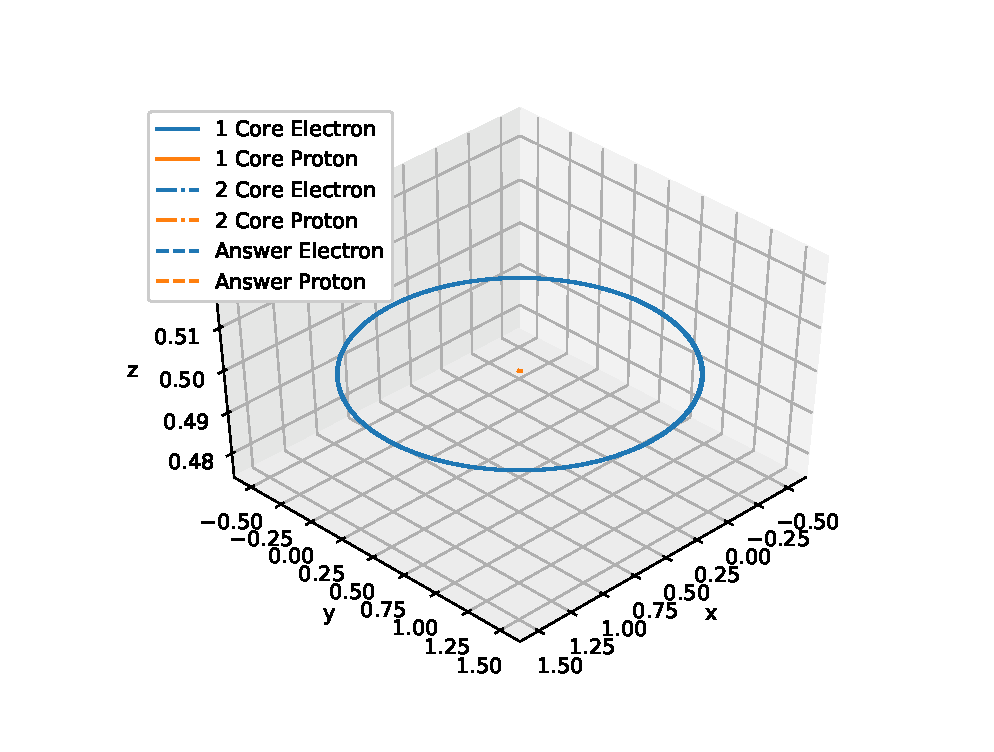
\includegraphics[width=8cm\linewidth, height=8cm\textheight]{Trajectory}
	\caption{Classical trajectory of an electron around a proton with dt=0.001, for both the single core and multi core case.}
	\label{fig:trajectory}
\end{figure}

\begin{figure}
	\centering
	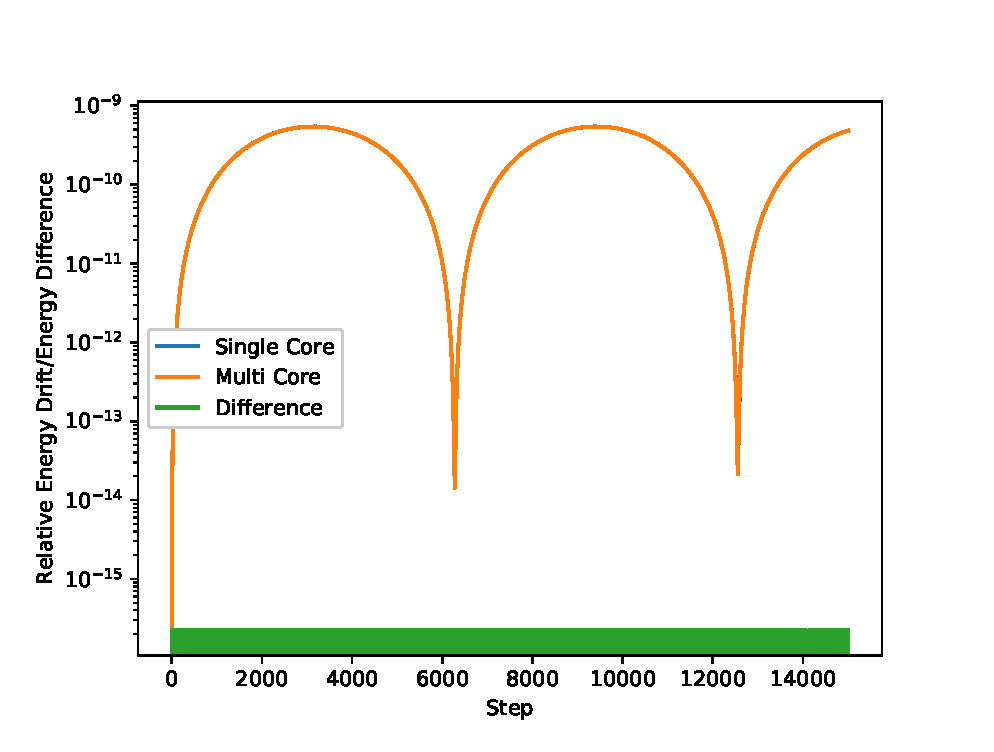
\includegraphics[width=9cm\linewidth, height=5cm\textheight]{Energy}
	\caption{A plot of the energy of the system relative to the initial energy. The green line shows the relative energy difference between the single core and multicore cases with respect to the initial single core energy.}
	\label{fig:energy}
\end{figure}

Both of these show that the integrator works properly and that there is no overcounting
of energy or forces. But just for safety an additional 100 particle test was run
to check energy conservation on a larger scale. This was done by running a random 
collection of 100 particles on a single core and on multiple cores. The energy results
for $dt=1e-3$ are shown in figure 3; the sudden jump in energy is characteristic of
collisions with low impact parameters. To show that this sudden jump disappears
in the limit of infinitesimal $dt$, the same plot shows the relative energy drift
for $dt=1e-4$. Clearly decreasing the timestep even further would limit the jump 
further. 

\begin{figure}
	\centering
	\includegraphics[width=8cm\linewidth, height=8cm\textheight]{NbodyEnergy}
	\caption{}
	\label{fig:nbodyenergy}
\end{figure}


\section{\label{sec:level1}Scaling}

Having confirmed energy conservation and proper trajectories, ppmd just needed scaling
tests, however, due to time and energy constraints, a large scale performance study was
not possible. Instead weak and strong scaling were both performed on an intel i6900k 
core on a robust local machine with 64 gb of DDR4 RAM. For the strong scaling test up to 9 ranks each
took a timestep for a single system of 1000 particles 5 times, and the average value
of each time step is shown in figure 4.

\begin{figure}
	\centering
	\includegraphics[width=8cm\linewidth, height=8cm\textheight]{StrongScaling}
	\caption{}
	\label{fig:strongscaling}
\end{figure}

The sudden jump in at $n_{ranks}=2$ could be attributed to a number of different 
phenomena depending on how the chip scheduling is done. Since the chip has 8
physical cores (16 hyper-threaded), it could be that the 2 rank test was split
between two physical cores with a high spatial separation, leading to a longer
net runtime. Other explanations include slowed memory accesses or a transition
from a single cache to multiple caches on the chip. The flatline at ranks=4 is
definitely explained by the transition to using all the resources of several
physical cores, before dropping even further with the use of every physical core.
Overall, for a constant problem, it scales fairly well in this small case. Obviously
a more rigorous testing study needs to be conducted at a much larger scale when
possible.

For the weak scaling, each rank was assigned 1000 particles. Obviously this is where
the direct force calculation completely breaks down, and the program loses all allure
from the user perspective due to poor performance, as shown in figure 5. The sharp up
tick at 5 ranks is again due to a transition to using all processors instead of hyperthreading only a few, but it doesn't scale well (as was expected).


\begin{figure}
	\centering
	\includegraphics[width=8cm\linewidth, height=8cm\textheight]{WeakScaling}
	\caption{}
	\label{fig:weakscaling}
\end{figure}

As far as memory scaling is concerned, it is linearly proportional to the total
number of processors. This means there is a critical point at which the program
will not run due to the fact that a single processor cannot store the total
data on its particles and the location and type data of another processors 
particles, this is the point at which the program becomes memory limited rather
than compute bound. 


\section{\label{sec:level1}Conclusions}
In this paper we have implemented an $\mathcal{O}(N^{2})$ purely python molecular dynamics code utilizing a velocity verlet integrator for systems with various
different boundary conditions. While an attempt at heterogeneous computing was
made, python ultimately made this endeavor more difficult than coding the problem
in a lower level systems language, and so that was abandoned. The code was
validated with two different tests demonstrating energy conservation and proper
dynamics on multiple cores. Strong scaling showed decent results and the weak scaling
of the code was atrocious, all of this without being done on a large system. 
Overall the project showed that developing in python does not give the level
of memory granularity and program control that would be desired in an hpc code,
and it depended highly on several external packages. The best path forward would
be to take the code design and rewrite it in c++ and then focus on developing an
efficient FMM force solver. 


\bibliography{citations.bib}
\end{document}
%
% ****** End of file apssamp.tex ******